\documentclass[norsk,8pt,a4paper]{report}
\usepackage[margin=1.5cm,tmargin=1.0cm,bmargin=1.0cm,rmargin=1.5cm,lmargin=1.5cm,footskip=0.2cm]{geometry}
\title{MAT101 - Innlevering 2 (Gruppe 16)}
\author{}
\date{}

% % % % % % % % % % % % % % % % % % % % % % % % % % % % % % % % % % % % % % % % 

\usepackage{babel}               % Support for other languages than english
\usepackage{setspace}            % Set paragraph spacing
\usepackage{nicefrac}            % Nice looking fractals
\usepackage{graphicx}            % Images
\usepackage{gensymb}             % Degree symbol
\usepackage{listings}            % Code
\usepackage{ulem}                % Double underline
\usepackage{amssymb}             % ...
\usepackage{pdfpages}            % Insert pdf pages
\usepackage{enumitem}            % Lists
\usepackage{colortbl}            % Colored tables
\usepackage[compact]{titlesec}   % ...
\usepackage[T1]{fontenc}         % ...
\usepackage[utf8]{inputenc}      % ...
\usepackage[fleqn]{amsmath}      % ...
\usepackage[makeroom]{cancel}    % ...
%\usepackage{empheq}              % ...
%\setstretch{1.5}
\setlength{\parindent}{0pt}
\titlespacing*{\subsection}{0cm}{1.5cm}{0.5cm}
\lstset{
aboveskip=0cm,
belowskip=0cm,
showstringspaces=false,
columns=flexible,
basicstyle={\scriptsize\ttfamily},
breaklines=true,
breakatwhitespace=true,
tabsize=4,
inputencoding = utf8,  % Input encoding
extendedchars = true,  % Extended ASCII
literate      =        % Support additional characters
{⋆}{{$\star\ $}}1 {∘}{{$\circ\ $}}1
{á}{{\'a}}1  {é}{{\'e}}1  {í}{{\'i}}1 {ó}{{\'o}}1  {ú}{{\'u}}1
{Á}{{\'A}}1  {É}{{\'E}}1  {Í}{{\'I}}1 {Ó}{{\'O}}1  {Ú}{{\'U}}1
{à}{{\`a}}1  {è}{{\`e}}1  {ì}{{\`i}}1 {ò}{{\`o}}1  {ù}{{\`u}}1
{À}{{\`A}}1  {È}{{\`E}}1  {Ì}{{\`I}}1 {Ò}{{\`O}}1  {Ù}{{\`U}}1
{ä}{{\"a}}1  {ë}{{\"e}}1  {ï}{{\"i}}1 {ö}{{\"o}}1  {ü}{{\"u}}1
{Ä}{{\"A}}1  {Ë}{{\"E}}1  {Ï}{{\"I}}1 {Ö}{{\"O}}1  {Ü}{{\"U}}1
{â}{{\^a}}1  {ê}{{\^e}}1  {î}{{\^i}}1 {ô}{{\^o}}1  {û}{{\^u}}1
{Â}{{\^A}}1  {Ê}{{\^E}}1  {Î}{{\^I}}1 {Ô}{{\^O}}1  {Û}{{\^U}}1
{œ}{{\oe}}1  {Œ}{{\OE}}1  {æ}{{\ae}}1 {Æ}{{\AE}}1  {ß}{{\ss}}1
{ẞ}{{\SS}}1  {ç}{{\c{c}}}1 {Ç}{{\c{C}}}1 {ø}{{\o}}1  {Ø}{{\O}}1
{å}{{\aa\ }}1  {Å}{{\AA}}1  {ã}{{\~a}}1  {õ}{{\~o}}1 {Ã}{{\~A}}1
{Õ}{{\~O}}1  {ñ}{{\~n}}1  {Ñ}{{\~N}}1  {¿}{{?`}}1  {¡}{{!`}}1
{„}{\quotedblbase}1 {“}{\textquotedblleft}1 {–}{$-$}1
{°}{{\textdegree}}1 {º}{{\textordmasculine}}1 {ª}{{\textordfeminine}}1
{£}{{\pounds}}1  {©}{{\copyright}}1  {®}{{\textregistered}}1
{«}{{\guillemotleft}}1  {»}{{\guillemotright}}1  {Ð}{{\DH}}1  {ð}{{\dh}}1
{Ý}{{\'Y}}1    {ý}{{\'y}}1    {Þ}{{\TH}}1    {þ}{{\th}}1    {Ă}{{\u{A}}}1
{ă}{{\u{a}}}1  {Ą}{{\k{A}}}1  {ą}{{\k{a}}}1  {Ć}{{\'C}}1    {ć}{{\'c}}1
{Č}{{\v{C}}}1  {č}{{\v{c}}}1  {Ď}{{\v{D}}}1  {ď}{{\v{d}}}1  {Đ}{{\DJ}}1
{đ}{{\dj}}1    {Ė}{{\.{E}}}1  {ė}{{\.{e}}}1  {Ę}{{\k{E}}}1  {ę}{{\k{e}}}1
{Ě}{{\v{E}}}1  {ě}{{\v{e}}}1  {Ğ}{{\u{G}}}1  {ğ}{{\u{g}}}1  {Ĩ}{{\~I}}1
{ĩ}{{\~\i}}1   {Į}{{\k{I}}}1  {į}{{\k{i}}}1  {İ}{{\.{I}}}1  {ı}{{\i}}1
{Ĺ}{{\'L}}1    {ĺ}{{\'l}}1    {Ľ}{{\v{L}}}1  {ľ}{{\v{l}}}1  {Ł}{{\L{}}}1
{ł}{{\l{}}}1   {Ń}{{\'N}}1    {ń}{{\'n}}1    {Ň}{{\v{N}}}1  {ň}{{\v{n}}}1
{Ő}{{\H{O}}}1  {ő}{{\H{o}}}1  {Ŕ}{{\'{R}}}1  {ŕ}{{\'{r}}}1  {Ř}{{\v{R}}}1
{ř}{{\v{r}}}1  {Ś}{{\'S}}1    {ś}{{\'s}}1    {Ş}{{\c{S}}}1  {ş}{{\c{s}}}1
{Š}{{\v{S}}}1  {š}{{\v{s}}}1  {Ť}{{\v{T}}}1  {ť}{{\v{t}}}1  {Ũ}{{\~U}}1
{ũ}{{\~u}}1    {Ū}{{\={U}}}1  {ū}{{\={u}}}1  {Ů}{{\r{U}}}1  {ů}{{\r{u}}}1
{Ű}{{\H{U}}}1  {ű}{{\H{u}}}1  {Ų}{{\k{U}}}1  {ų}{{\k{u}}}1  {Ź}{{\'Z}}1
{ź}{{\'z}}1    {Ż}{{\.Z}}1    {ż}{{\.z}}1    {Ž}{{\v{Z}}}1  {ž}{{\v{z}}}1
}

\newlength{\myeqskip}  \setlength{\myeqskip}{2pt}
\AtBeginDocument{%
    \setlength\abovedisplayskip{\myeqskip}%
    \setlength\belowdisplayskip{\myeqskip}%
    \setlength\abovedisplayshortskip{\myeqskip-\baselineskip}%
    \setlength\belowdisplayshortskip{\myeqskip}}

% % % % % % % % % % % % % % % % % % % % % % % % % % % % % % % % % % % % % % % % 

\newcommand{\oppgave}[1]{\subsection*{Oppgave #1}}
\newcommand{\oppgaveDelStart}{\begin{enumerate}[leftmargin=*,itemsep=1.5cm,labelsep=1.5em,label=\alph*)]}
\newcommand{\oppgaveDelSlutt}{\end{enumerate}}
\newcommand{\oppgaveDel}[1]{\item[#1)]}

% % % % % % % % % % % % % % % % % % % % % % % % % % % % % % % % % % % % % % % % 

\begin{document}

% % % % % % % % % % % % % % % % % % % % % % % % % % % % % % % % % % % % % % % % 

\oppgave{1}
\begin{align*}
G &= \{ 2, 3, 4, 5, 6 \}\\
A \cup B &= \{ 2, 3, 4, 5 \}\\
A^C &= \{ 2, 4, 6 \}\\
A \setminus B &= \{ 5 \}\\
A \cup A^C &= G\\
A &= G - A^C\\
A &= \{ 2, 3, 4, 5, 6 \} - \{ 2, 4, 6 \}\\
\Rightarrow A &= \uuline{ \{ 3,5 \} }\\
(A - B) \cup B &= A \cup B\\
\{ 5 \} \cup B &= \{ 2,3,4,5 \}\\
\Rightarrow B &= \uuline{\{ 2,3,4 \}}\\
\end{align*}

% % % % % % % % % % % % % % % % % % % % % % % % % % % % % % % % % % % % % % % % 

\oppgave{2}
%\begin{align*}
%&(A - B) \cap (C - B) = A - (B \cup C)\\
%\end{align*}
\oppgaveDelStart
\oppgaveDel{a}
\begin{align*}
\text{Let } A &= \{ 1,2,3,4 \}\\
B &=\{ 1,2 \}\\
C &=\{ 1,2,3 \}\\
\text{Then }A -B &=\{ 3,4 \}\\
C - B&=\{ 3 \}\\
B \cup C &=\{ 1,2,3 \}\\
\Rightarrow (A - B) \cap (C - B) &=\{ 3 \}\\
\text{And } A - (B \cup C) &=\{ 4 \}\\
\{ 3 \} &\neq\{ 4 \}\\
(A - B) \cap (C - B) &\neq A - (B \cup C)\\
\end{align*}

\oppgaveDel{b}
\begin{align*}
(1)\ X - Y &= X \cap Y^C\\
X - Y &= \{ x \mid x \in X \text{ and } x \not\in Y \}\\
X - Y &= \{ x \mid x \in X \text{ and } x \in Y^C \}\\\\
(2)\  B^C - A\\
(2) \text{ inn i } (1)\  B^C - A &= B^C \cap A^C \\\\
(B^C \cup (B^C - A))^C &= (B^C \cup (B^C \cap A^C))^C\\
(B^C \cup (B^C \cap A^C))^C &= ( (B^C \cup B^C) \cap (B^C \cup A^C) )^C &&\text{[Distribusjonslov]}\\
( (B^C \cup B^C) \cap (B^C \cup A^C) )^C &= ( B^C \cap (B^C \cup A^C) )^C\\
( B^C \cap (B^C \cup A^C) )^C &= (B^C)^C &&\text{[Absorbsjonslov]}\\
(B^C)^C &= B\\
\end{align*}

\oppgaveDelSlutt

% % % % % % % % % % % % % % % % % % % % % % % % % % % % % % % % % % % % % % % % 

\oppgave{3}
\oppgaveDelStart
\oppgaveDel{a}
\begin{align*}
&\{ a \} \cap \{ c \} = \emptyset\\
&\mathcal{J} \text{ holder ikke.}\\
\end{align*}

\oppgaveDel{b}
\begin{align*}
&\{ a, b \} \cap \{ a, b, c \} = \{ a, b \}\\
&\mathcal{J} \text{ holder.}\\
\end{align*}

\oppgaveDelSlutt

% % % % % % % % % % % % % % % % % % % % % % % % % % % % % % % % % % % % % % % % 

\oppgave{4}
\oppgaveDelStart
\oppgaveDel{a}
\begin{align*}
&2x - 2y = 2(x-y)\\
&\text{Det betyr at,}\\
&\text{hvis } x-y=1 \text{, da blir } 2(x-y) = 2(1) = 2 \in A,\\
&\text{hvis } x-y=2 \text{, da blir } 2(x-y) = 2(2) = 4 \in A,\\
&\text{hvis } x-y=3 \text{, da blir } 2(x-y) = 2(3) = 6 \not\in A.\\
&\text{Derfor må vi finne tupler der } x-y = 1 \text{ eller } x-y =2.\\
&\text{For } x-y = 1 : (2,1), (3,2), (4,3), (5,4)\\
&\text{Og for } x-y = 2: (3,1), (4,2), (5,3)\\
&\text{Dette gir mengden for relasjonen} \sim :\\
&\Big\{(2,1), (3,2), (4,3), (5,4), (3,1), (4,2), (5,3) \Big\}\\
\end{align*}

\oppgaveDel{b}
\parbox{\linewidth}{\centering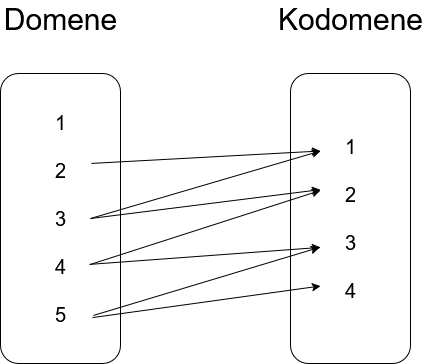
\includegraphics[width=0.4\linewidth]{4b.png}}

\oppgaveDel{c}
Nei, $\sim$ er ikke en funksjon.\\
- Elementet 1 fra domenet er ikke i relasjon med et annet element.\\
- Elementene 3, 4 og 5 fra domenet er i relasjon med to elementer i kodomenet.

\oppgaveDelSlutt

\newpage

\oppgave{4}
\oppgaveDelStart

\oppgaveDel{d}
Er relasjonen refleksiv?\\
$x \sim x = 2(x-x) = 0 \not\in A$\\
Relasjonen er \uline{ikke refleksiv}.\\\\

Er relasjonen symmetrisk?\\
Hvis $x \sim y$, da er $2(x-y) \in A$,\\
for at relasjonen skal være symmetrisk må også,\\
$y \sim x$ som tilsier at $2(y-x) \in A$,\\
men $2(y-x) = -2(x-y)$ som aldri vil holde for $\sim$,\\
siden det alltid vil gi en negativ verdi, og det er ikke et element i $A$.\\\\

Er relasjonen antisymmetrisk?
???\\\\

Er relasjonen transitiv?
\begin{align*}
\text{Hvis }5 \sim 2 \text{ og } 4 \sim 2 \Rightarrow 5 \sim 2\\
2(5-4) = 1 \in A\\
2(4-2) = 2 \in A\\
2(5-2) = 6 \not\in A\\
\end{align*}
\text{Moteksempel viser at relasjonen \uline{ikke er transitiv}.}

\oppgaveDel{e}
Dette er ikke en ekvivalensrelasjon, siden relasjonen ikke er refleksiv, eller symmetrisk, og oppfølger derfor ikke kravene for ekvivalensrelasjon.

\oppgaveDelSlutt

% % % % % % % % % % % % % % % % % % % % % % % % % % % % % % % % % % % % % % % % 


\oppgave{5}
\oppgaveDelStart
\oppgaveDel{a}
\ \\
i)\\
\begin{align*}
f(1) &= 2\\
f(2) &= 2\\
f(3) &= 6\\
f(4) &= 4\\
f(5) &= 10\\
f[A] &= \{ 2, 4, 6, 10\}\\\\
f(2) &= 2\\
f(6) &= 6\\
f(8) &= 8\\
f(10) &= 10\\
f[B] &= \{ 2, 6, 8, 10 \} = B\\
\end{align*}
\oppgaveDelSlutt

\newpage

\oppgave{5}
\oppgaveDelStart
\oppgaveDel{a}
\ \\
ii)\\

\begin{align*}
f(1) &= 2\\
f(2) &= 2\\
\end{align*}
Dette tilsier at $f$ ikke er injektiv, siden to elementer fra domene gir samme element i kodomenet.\\
Ettersom $f$ ikke er injektiv er $f$ heller ikke bijektiv.

\oppgaveDel{b}
\lstinputlisting[language=Haskell]{q5b.hs}

\oppgaveDelSlutt

% % % % % % % % % % % % % % % % % % % % % % % % % % % % % % % % % % % % % % % % 


\oppgave{6}
\oppgaveDelStart
\lstinputlisting[language=Haskell]{q6.hs}
\oppgaveDelSlutt

% % % % % % % % % % % % % % % % % % % % % % % % % % % % % % % % % % % % % % % % 

\oppgave{7}
\oppgaveDelStart
\oppgaveDelSlutt

% % % % % % % % % % % % % % % % % % % % % % % % % % % % % % % % % % % % % % % % 

\end{document}

